%%%
%%% OpenCAEシンポジウムTeXテンプレートファイル
%%% OpenFAOM-jp_OpenCAE_symposium.tex
%%% OpenCAEシンポジウム2018版
%%%
%%
%% ltjocはOpenCAE論文集・シンポジウム用のクラスファイルです.変更しないでください.
%% 本文が英語の場合には,オプションにenglishを指定してください.
\documentclass{ltjoc}
%\documentclass[english]{ltjoc}
%%
%% 表題(title),副題(subtitle),著者(author),所属(affiliation)
%% 本文が英語の場合には,こちらに英文表題,英文副題,英文著者,英文所属を記述します.
\title{OpenFOAMコントリビュート活動}
% 副題が無い場合にはコメントアウトします.
% \subtitle{\TeX のテンプレート(和文副題)} 
\author{%
@public\_inabower$^{1\dagger}$%
\hspace{1\zw}%
松原 大輔$^{2}$%
\hspace{1\zw}%
@tkoyama010$^{1}$%
}
\affiliation{%
${}^{1}$OpenFOAM-jp%
\hspace{1\zw}%
${}^{2}$オープン CAE勉強会%
} 
%%
%% Corresponding authorの電子メールアドレス
%% 本論文について連絡が取れる著者の電子メールアドレスを記載してください.
\AuthorsEmail{office@opencae.or.jp}
%%
%% 英文表題(etitle),英文副題(esubtitle),英文著者(eauthor),英文所属(eaffiliation)
%% 本文が英語の場合には表示されません.
\etitle{OpenFOAM Contributing Activities}
% 副題が無い場合にはコメントアウトします.
% \esubtitle{The case of \TeX (English Sub-Title)}
\eauthor{%
@public\_inabower$^{*\dagger}$%
\hspace{1em}%
Daisuke MATSUBARA$^{**}$%
\hspace{1em}%
@tkoyama010$^{*}$%
}
\eaffiliation{%
${}^{*}$OpenFOAM-jp%
\hspace{1em}%
${}^{**}$OpenCAE Local user group%
}
%%
%% キーワード
\keywords{Keyword1, Keyword2, Keyword3, Keyword4, Keyword5}
%%
%% 英文概要
%% 英文概要を省略する場合には,abstract環境の定義をしないでください.
\begin{abstract}
The quick brown fox jumps over the lazy dog.
The quick brown fox jumps over the lazy dog.
The quick brown fox jumps over the lazy dog.
The quick brown fox jumps over the lazy dog.
The quick brown fox jumps over the lazy dog.
The quick brown fox jumps over the lazy dog.
\end{abstract}
%%
%% luatexja-fontspecパッケージ
\usepackage{luatexja-fontspec}
\defaultfontfeatures{Ligatures=TeX}
%% luatexja-presetパッケージ
%% 和文フォントのプリセット設定
%% オプションにnoembed(非埋込)を指定しないでください.
%\usepackage[ipaex]{luatexja-preset} % IPAex(デフォルト)
%\usepackage[ms]{luatexja-preset} % MS
%\usepackage[hiragino-pro]{luatexja-preset} % ヒラギノPro
%%
%% 欧文フォントの指定
%% 使用できるフォントについては,以下のコマンドで調べてください.
%% $ luaotfload-tool --list=*
%%
%% 欧文通常フォント
%\setmainfont{Cambria} % Cambria
%\setmainfont{Times New Roman} % Times New Roman
%\setmainfont{TeXGyreTermes} % TeXGyreTermes
%%
%% 欧文Sans-serifフォント
%\setsansfont{Calibri} % Calibri
%\setsansfont{Arial} % Arial
%\setsansfont{Helvetica} % Helvetica
%\setsansfont{TeXGyreHeros} % TeXGyreHeros
%%
%% 欧文monospaceフォント
%\setmonofont{Consolas} % Consolas
%\setmonofont{Courier New} % Courier New
%\setmonofont{Lucida Console} % Lucida Console
%%
%% subfigureパッケージ
\usepackage{subfigure}
%%
%% graphicxパッケージ
\usepackage{graphicx}
%%
%% hyperrefパッケージ
\usepackage[
 pdfencoding=auto,
 bookmarks=true,
 bookmarksnumbered=true,
 colorlinks=true,
 allcolors={blue}
]{hyperref}
%%
%% listingsパッケージ
\usepackage{listings}
\renewcommand{\lstlistingname}{Code}
\lstset{
basicstyle={\footnotesize\ttfamily},
commentstyle=\color{blue},
frame={tb},
breaklines=true,
columns=[l]{fullflexible},
numbers=left,
numberstyle={\footnotesize},
keepspaces=true
}
%%
%% autorefでの図表の参照名の再定義
\makeatletter
\if@english
  \renewcommand*{\figureautorefname}{\figurename}
  \renewcommand*{\tableautorefname}{\tablename}
\else
  \renewcommand*{\figureautorefname}{図}
  \renewcommand*{\tableautorefname}{表}
\fi
\makeatother
%%
%% ヘッダ右の設定
%% 変更しないでください.
\markright{Open CAE Symposium 2018, Dec. 7-8, 2018, Kawasaki} % Do not edit this line
%%
%% 本文
\begin{document}
%%
%% 題目などの出力
\maketitle
%%%
\section{はじめに}
\section{ESI版とFoundation版の違い}
\section{ESI版コントリビュート方法}
\section{Foundation版コントリビュート方法}

Foundation版は基本的にbugfixを目的としたコントリビュートが主であるため,バグ報告を行うためのissueTrackingのページへ登録する必要がある.
未登録の場合は,名前とメールアドレスを入力し,返信のリンクを辿ることでviewerとして参加することができる.
また数時間後にスパムでないことが認められると,reporterに昇格できる.
reporterとなることでissueを立てて,バグの報告が可能となる.
ここで本当にバグなのか,改善する方法はあるのかなどを議論することになる.

重大なバグの修正または,新しい開発を提供する場合,OpenFOAM Foundation Contributor Agreementに署名する必要がある.
Foundation版HPのメニューバーのDevelopment/ContributorAgreeementのリンクを辿り,Contact Usのページから名前と所属,コントリビュートに参加した意思を記載して送信すると,後日,Henry G. WellerからPDF形式の登録用紙が送付されてくる.
登録用紙の内容は,前述のContributorAgreeementのページに記載されているものと同じである.

バグの修正などでFoundation版のOpenFOAMの修正を開発元に共有する場合,Foundation版のOpenFOAMはgithub上で管理されているため,githubアカウントが必要となる.

コントリビュートで最初に行うことは開発元のリポジトリをForkすることから始まる.
Forkしたことにより,自身のgithubアカウントにOpenFOAMのリポジトリが作成されていることが確認できる.
次に開発用の新しいブランチを作成する.ブランチ名は「(開発者名)-patch***」などとするとよいだろう.今回の例では「matsubara-patch1」とした.

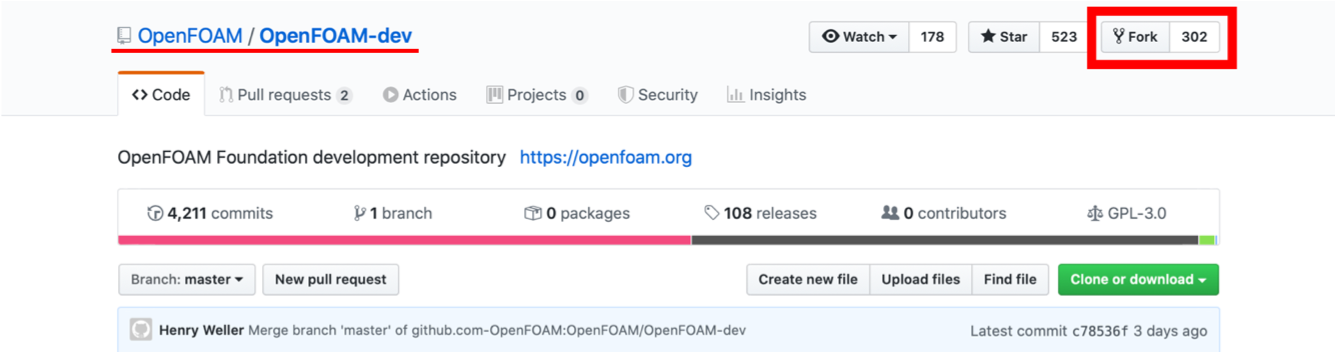
\includegraphics[width=5cm]{fig/fig-f1.png}
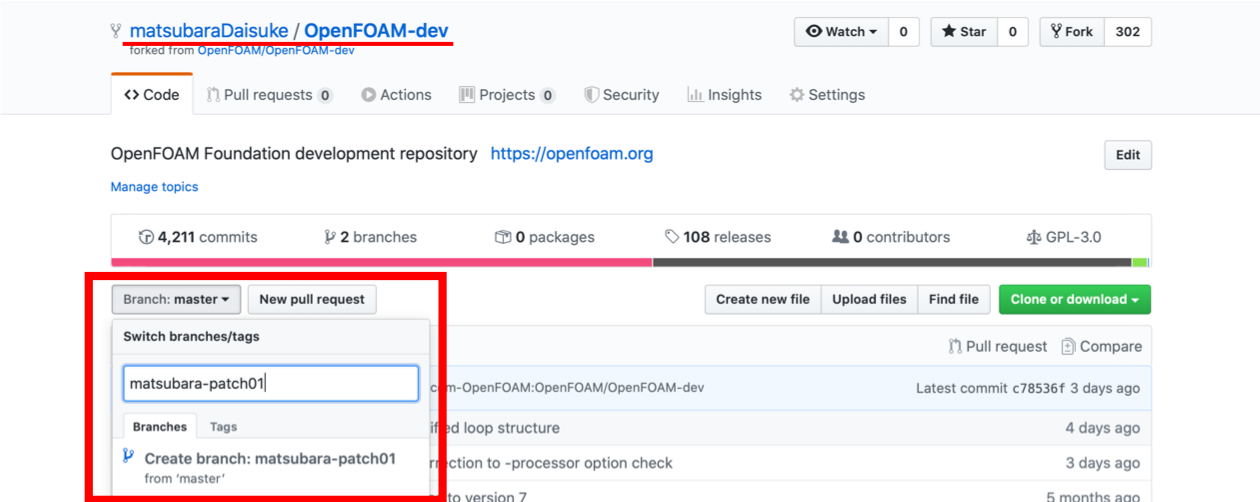
\includegraphics[width=5cm]{fig/fig-f2.png}

次に個人の開発環境に移りターミナル上でgit cloneを行う.例:git clone https://github.com/(githubアカウント名)/OpenFOAM-dev.git
これによって,git cloneしたディレクトリ下にOpenFOAMのプロジェクトがコピーされる.
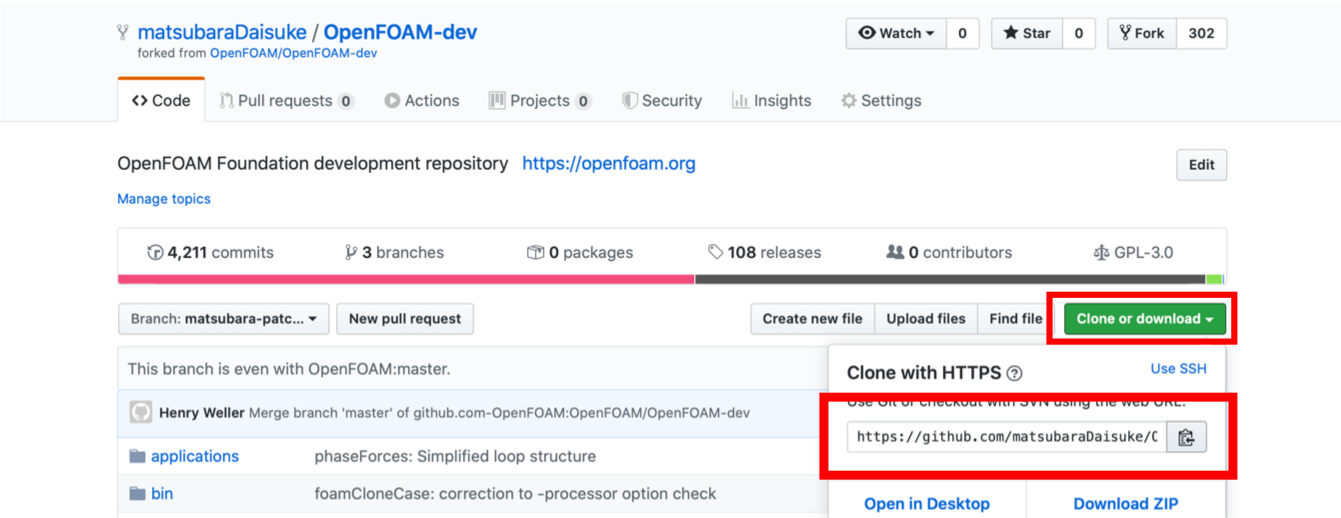
\includegraphics[width=5cm]{fig/fig-f3.png}

次にgit checkoutにて作成したブランチに切り替える 例:git checkout (開発者名)-patch***
OpenFOAMのプロジェクト内で修正や開発が完了した後,
git add . git commit -m "変更内容のコメント" git push origin (開発者名)-patch***
とすることで,コードの修正内容を個人のgithubのリポジトリに反映させる.
今回の例では以下の様な流れになる.

\begin{shbox}
  \shuser{user}
  \shline{}{git clone https://github.com/matsubaraDaisuke/OpenFOAM-dev.git}  
  \shline{}{cd OpenFOAM-dev}  
  \shline{}{git checkout matsubara-patch1}
\end{shbox}

(コーディング)

\begin{shbox}
  \shuser{user}
  \shline{}{git add .}
  \shline{}{git commit -m "bugfix ******"}
  \shline{}{git push origin matsubara-patch1}
\end{shbox}



最後にgithub上でpull requestを開発元に対して行う.この時コメントに
Fixes issue:
https://bugs.openfoam.org/view.php?id=****
の様に最初に議論したissueのURLを添付するのが慣例のようである.

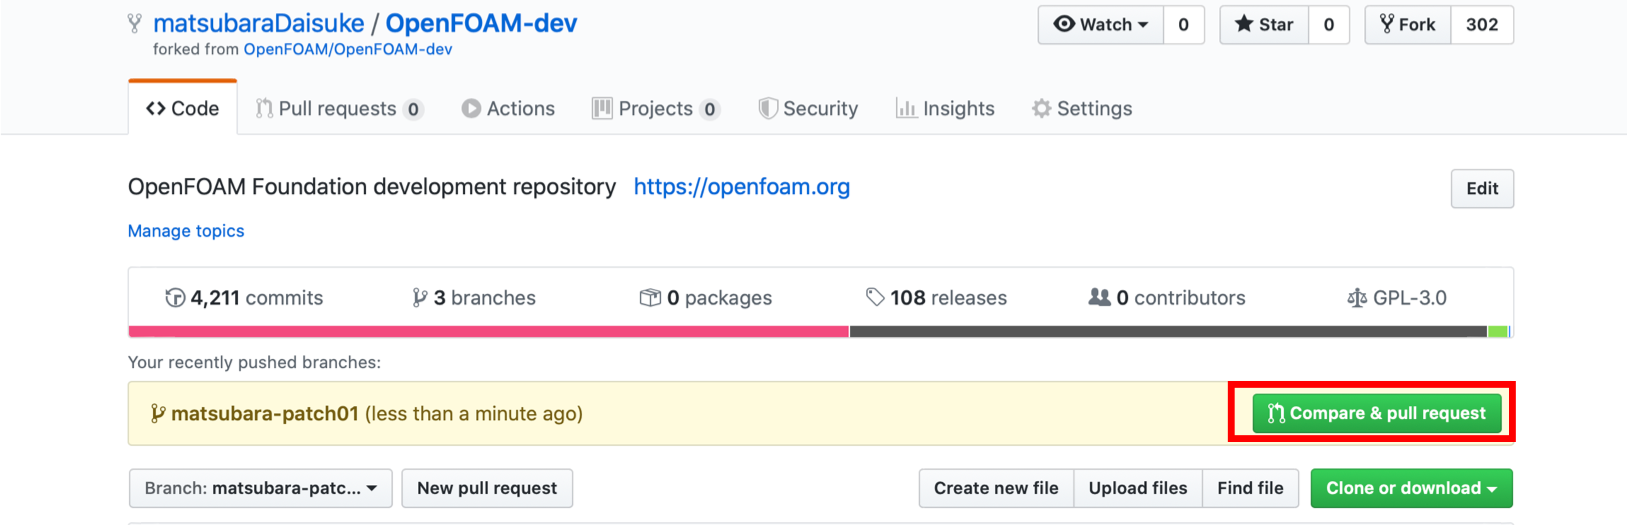
\includegraphics[width=5cm]{fig/fig-f4.png}
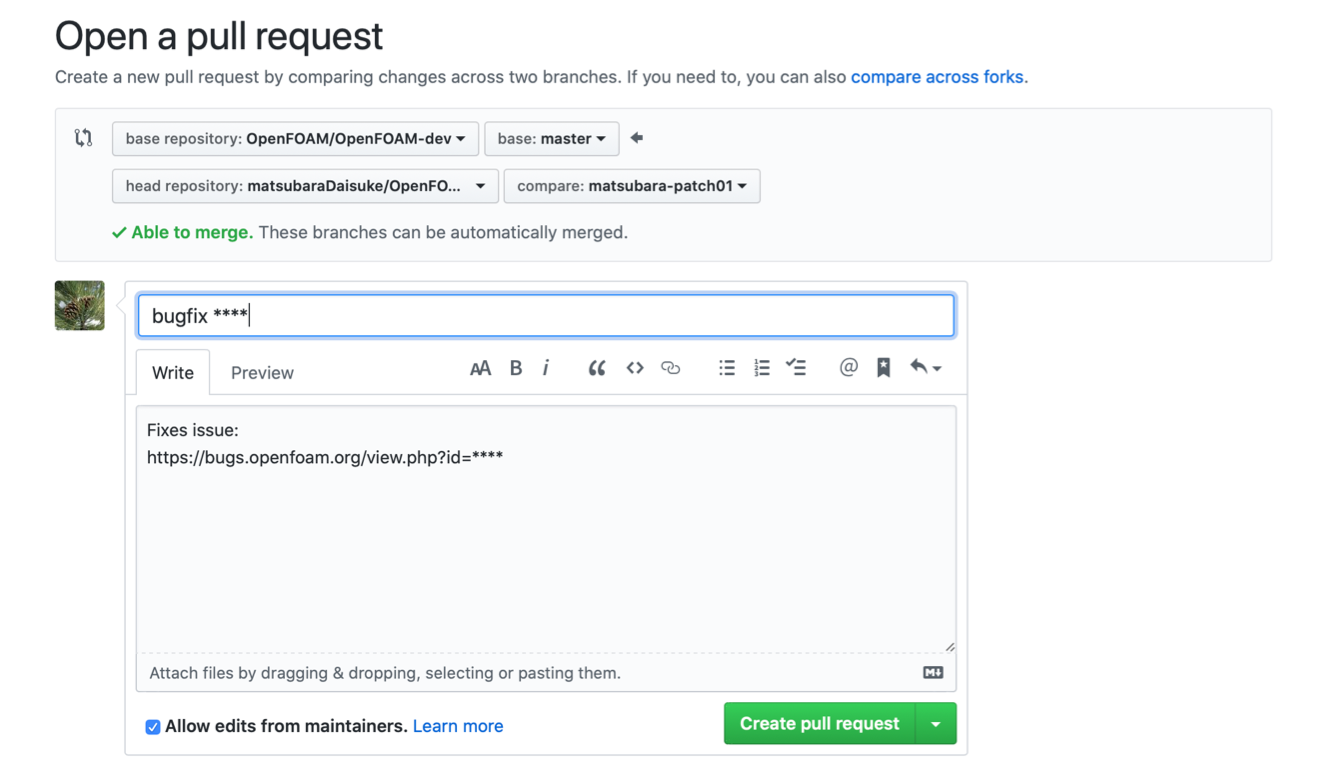
\includegraphics[width=5cm]{fig/fig-f5.png}


\section{Gitの使い方}
\section{GitHub および Travis による継続的インテグレーション}
\section{まとめ}
\end{document}
